\documentclass[11pt
  , a4paper
  , article
  , oneside
  %  , twoside
  , showtrims
 % , draft
]{memoir}

\usepackage{essdocs}
\usepackage[numbers]{natbib}
\usepackage[autostyle]{csquotes}

\setsecnumdepth{subsection}


\begin{document}
%\frontmatter
% ESS Document Description
%
\essdoctype{Engineering Manual}

% ESS Document Number
%
\essdocnum{ESS-0331569}

% Date
%
\date{\today}

% ESS Document Revision Number
%
\essdocrev{1}

% ESS Document State
%
\essdocstate{Released}

% ESS Document Classification
%
\essdocclass{Internal}

% Document Title
%
\title{ICS Engineering Manual}
\subtitle{for MRF MTCA-EVM-300}
% Document Author(s), if more than one author,
% use \newline instead of \\ or \linebreak in order to seperate them
\author{Javier Cereijo Garcia}
\authorrole{Timing System Engineer}

% Document Reviewer(s) if more than one reviewer,
% use \newline instead of \\ or \linebreak in order to seperate them
%\reviewer{-}
%\reviewerrole{-}

% Document Owner(s) if more than one owner,
% use \newline instead of \\ or \linebreak in order to seperate them
\owner{Javier Cereijo Garcia}
\ownerrole{Timing System Engineer}

% Document Approver(s) if more than one approver,
% use \newline instead of \\ or \linebreak in order to seperate them
%\approver{-}
%\approverrole{-}


\showtrimson

\esstitle
\newpage
\tableofcontents
\newpage

%\mainmatter


% Actual Document Start at below
\chapter{Overview}
At European Spallation Source (ESS), the Integrated Control System (ICS) uses the Micro-Research Finland (MRF) timing system{\footnote{\url{http://www.mrf.fi/}}} as its timing system of the ESS site. The consistent and up-to-date engineering manual is essential for the ESS timing system.\\


\section{Scope}
\begin{itemize}
\item This document identifies the Event Master (EVM) that is the backbone of the MRF timing system used to deliver synchronous frequencies, trigger signals and sequences of events \cite{MRFEVENTGENERATOR} to the ESS facility.
\item This document provides the generic description of the MRF mTCA-EVM-300. In addition, it affords the minimal, essential, and generic information for the system configuration.
\item The purpose of this document is to describe the engineering procedure and troubleshooting about how the MRF mTCA-EVM-300 board will be integrated in cooperation with the new ESS EPICS environment (E3).
\item This document attempts to maintain consistency with existing ESS Timing system hardware as far as possible.
\end{itemize}
%\textbf{Note that this is a very early draft document and should be updated as development progresses.}

\section{Target audience}
This document is targeted to ICS engineers and technical stakeholders of the ESS timing system. It is assumed that the target audience has a technical background in the MRF timing system, the Experimental Physics and Industrial Control System (EPICS) development, and a Linux environment.\\

\chapter{System description}
MRF Technical Reference document \citep[see][p12]{MRFEVENTGENERATOR} describes event generators (EVMs) as:
\blockquote{\textit{The Event Generator is responsible of creating and sending out timing events to an array of Event Receivers.
High configurability makes it feasible to build a whole timing system with a single Event Generator without external counters etc.\\
Events are sent out by the event generator as event frames (words) which consist of an eight bit event code and an eight bit distributed bus data byte. The event transfer rate is derived from an external RF clock or optionally an on-board clock generator. The optical event stream transmitted by the Event Generator is phase locked to the clock reference.\\
There are several sources of events: trigger events, sequence events, software events and events received from an upstream Event Generator. Events from different sources have different priority which is resolved in a priority encoder.\\
In addition to events the Event Generator enables the distribution of eight simultaneous signals sampled with the event clock rate, the distributed bus. Distributed bus signals may be provided externally or generated on-board by programmable multiplexed counters.}}

The scope of this document is to cover the mTCA-EVM-300 board.\\


\section{mTCA-EVM-300}
Figure~\ref{fig:mtcaevm300} shows the mTCA-EVM-300 card with rough physical dimensions $181\times 148~\mathrm{mm}{}^2$. The mTCA-EVM-300 has a small form-factor pluggable (SFP) transceiver as an output to fan-outs or Event Receivers (EVRs), one trigger input and one radio-frequency (RF) input.\\

\begin{figure}[!htb]
  \centering
  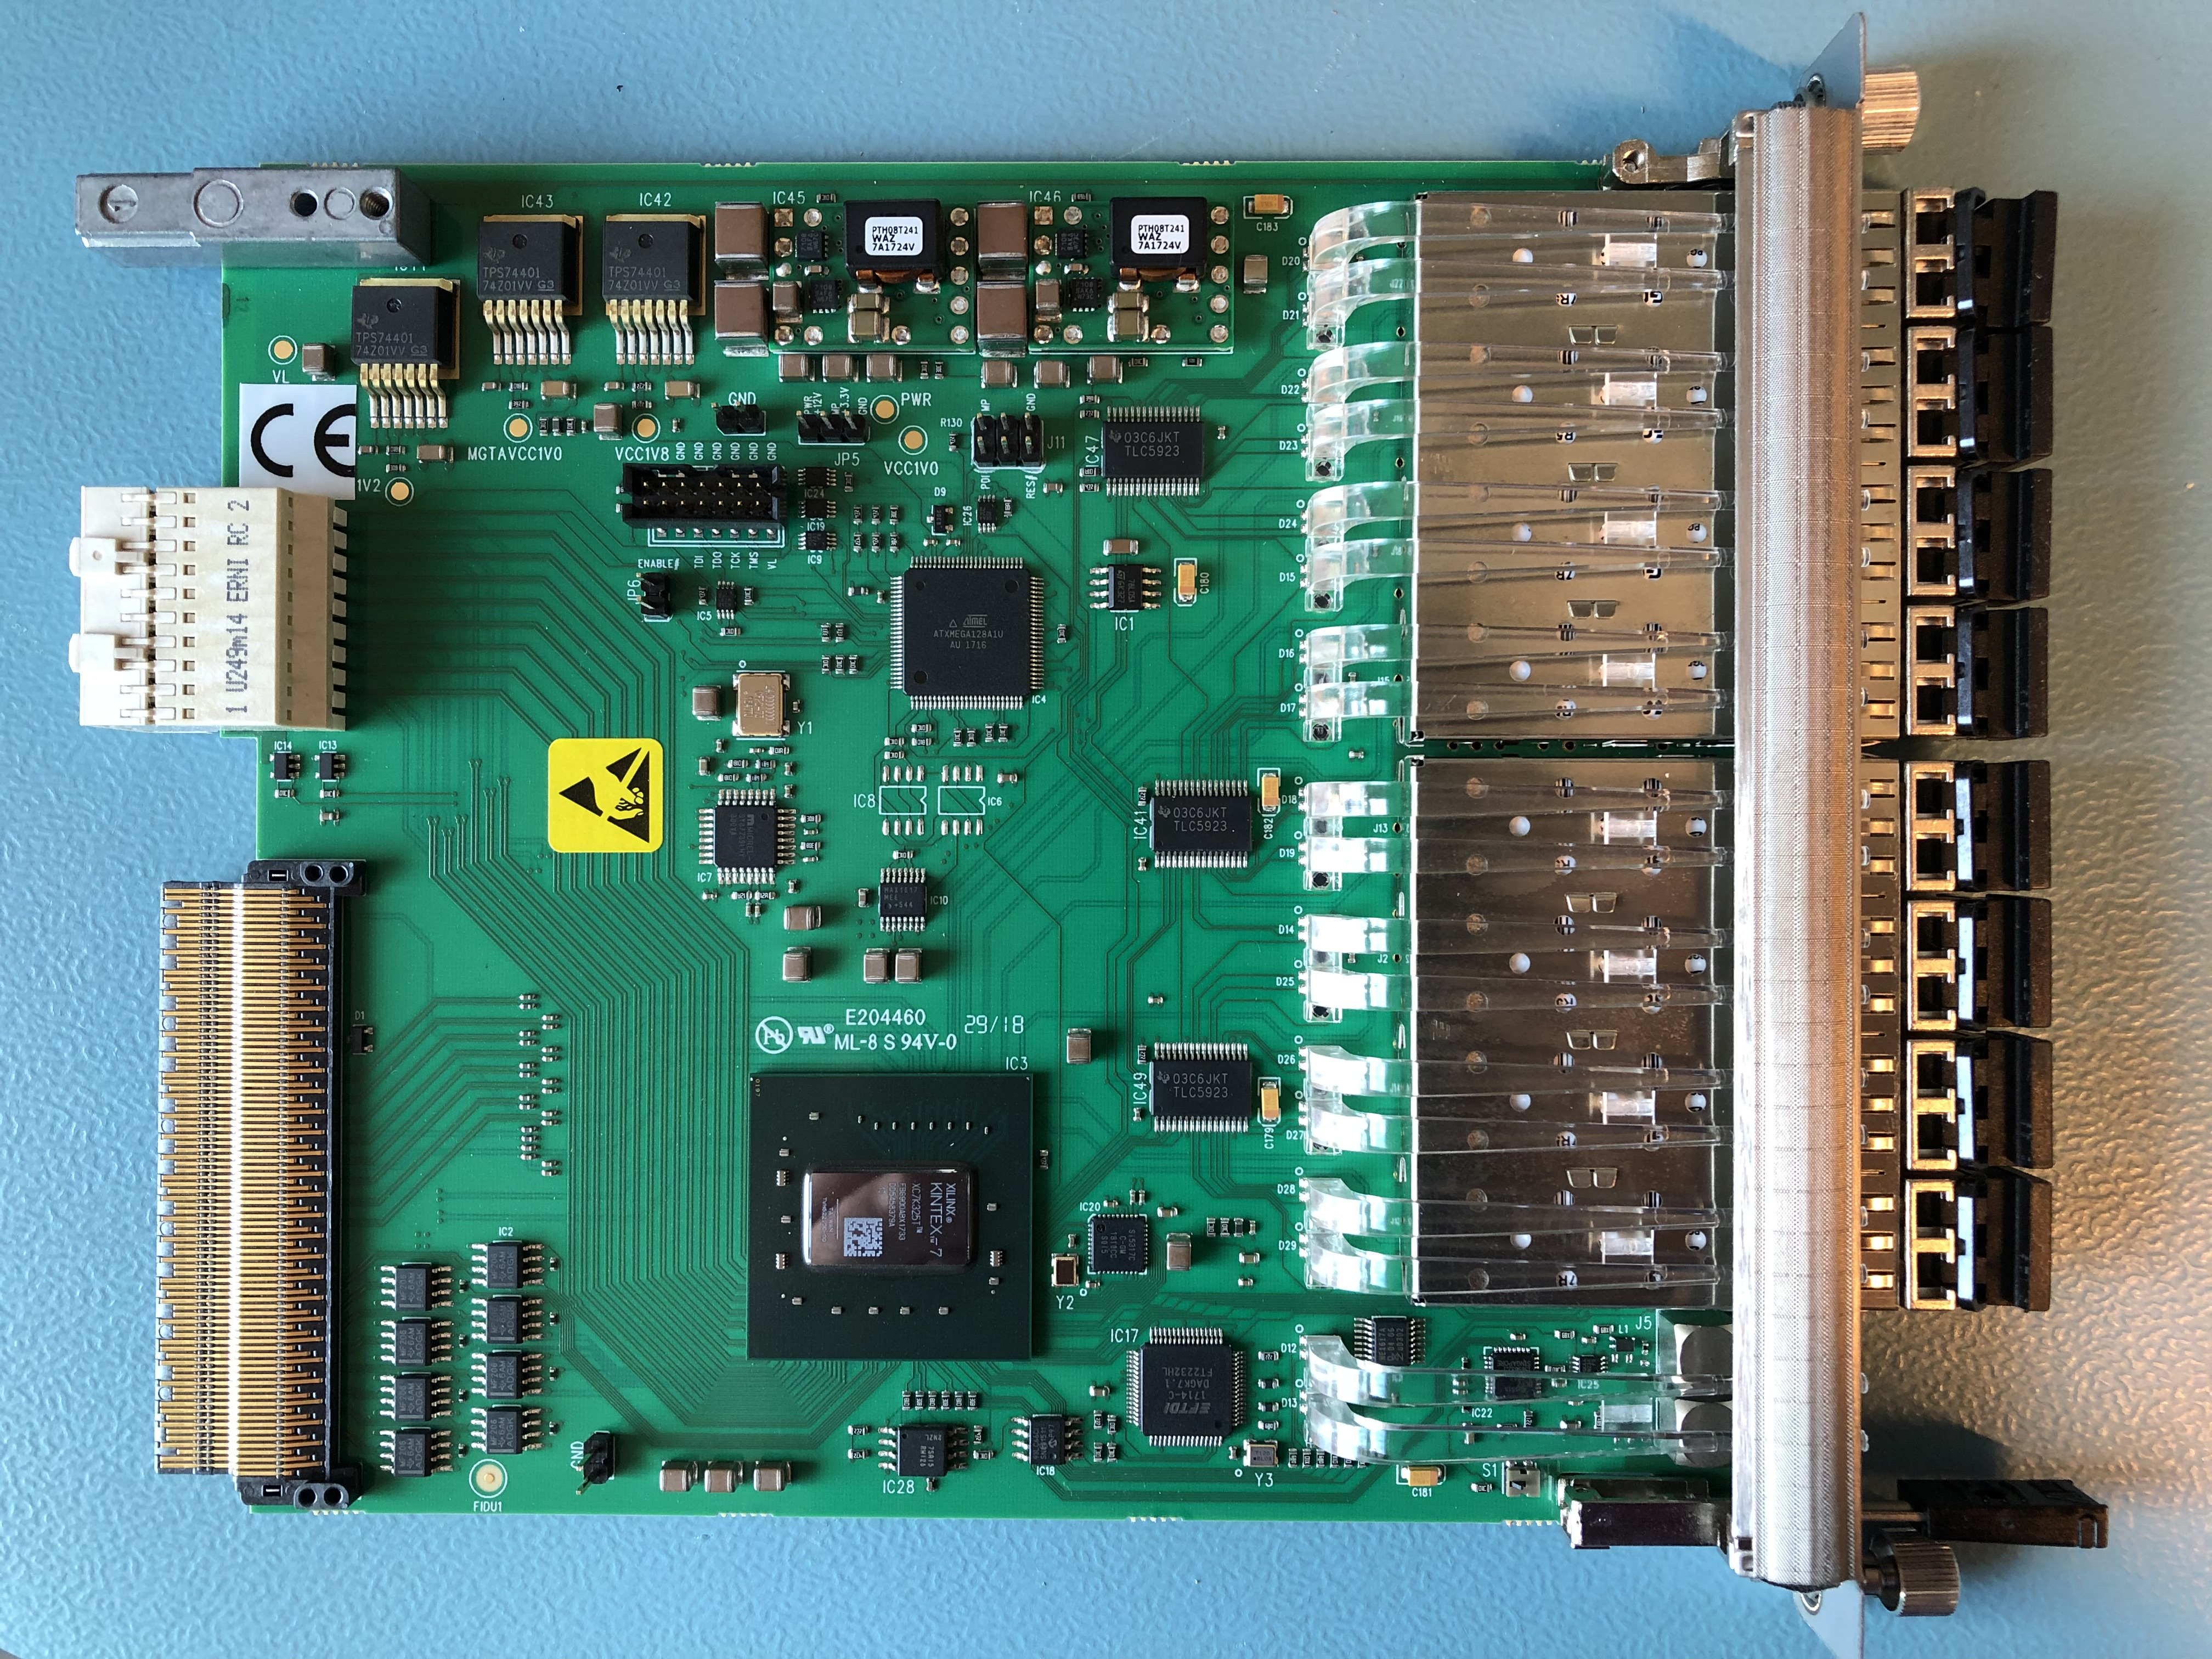
\includegraphics[width=0.99\textwidth]{./pictures/mTCA-EVM-300.jpg}
  \caption{MRF mTCA-EVM-300.}
  \label{fig:mtcaevm300}
\end{figure}


%\clearpage

\chapter{System environment}
Before describing the engineering procedure for the E3 integration of the MRF mTCA-EVM-300 board, it is mandatory to have a proper system environment that consists of specific hardware and software. Here we will show the hardware and software lists and their set up in the ICS lab at ESS. The information shown in this chapter is used in the ICS lab at ESS.\\


\section{Hardware}
Table~\ref{table:hwlist} shows the hardware list and its environment. It is possible to use a different form factor for the EVR than what is shown; for more information check the specific engineering manual.\\

\begin{table}[!hb]
  \centering
  \begin{tabular}{l|l}
    \toprule
    Hardware                        & Info                            \\\midrule
    MRF mTCA-EVM-300                &                                 \\\midrule
    MRF mTCA-EVR-300U               &                                 \\\midrule
    $\mu$TCA crate                  & Incl. PM, MCH                   \\\midrule
    Concurrent Technologies AMC CPU &                                 \\\midrule
    Optical cables                  & LC, optical 850 nm              \\\bottomrule
  \end{tabular}
  \caption[]{Hardware List.}
  \label{table:hwlist}
\end{table}

Figure~\ref{fig:evm-hw-setup} shows the mTCA-EVM-300 set up in the lab. From left to right, the power supply, MTCA Carrier Hub (MCH), Central Processing Unit (CPU) and mTCA-EVM-300.\\

\begin{figure}[!b]
  \centering
  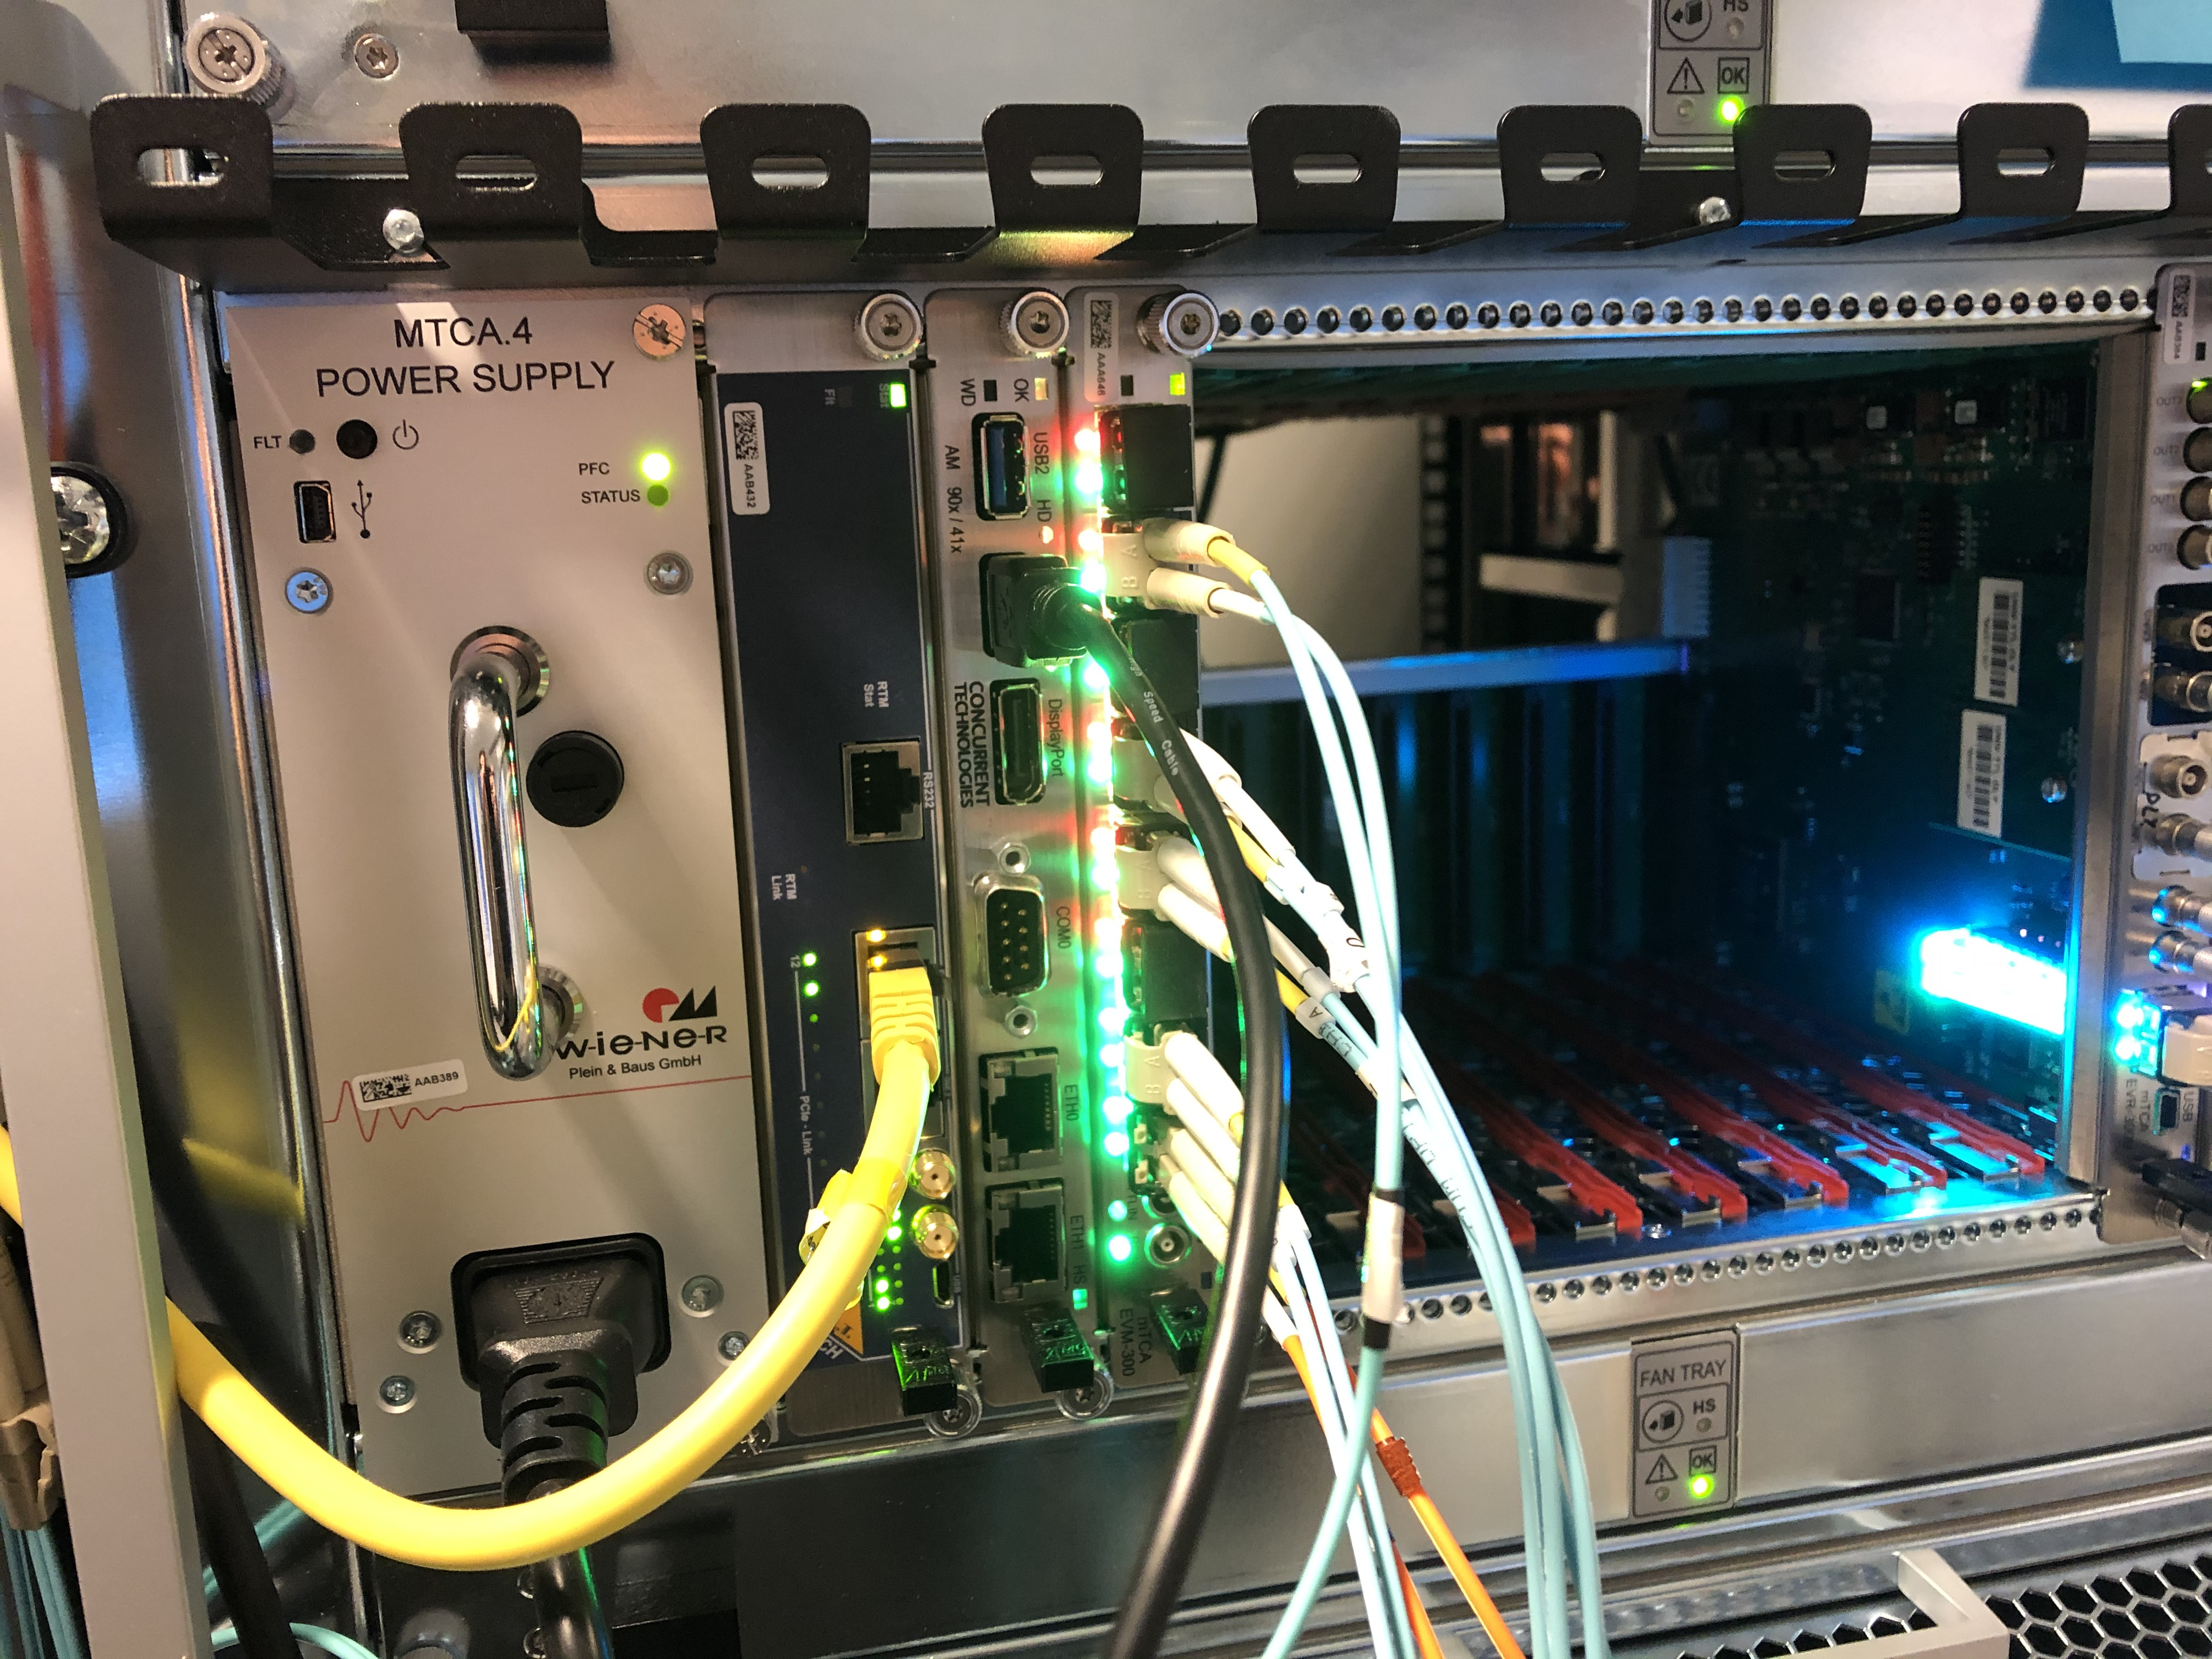
\includegraphics[width=0.8\textwidth]{./pictures/evm-hw-setup.jpg}
  \caption{Hardware set up in the ICS lab.}
  \label{fig:evm-hw-setup}
\end{figure}


%\clearpage
\section{Software}
Table~\ref{table:swlist} shows the Software list and its environment. It is mandatory to check the kernel version, and the mrf kernel module version. Since the mrfioc2 is dependent upon devlib2 E3 internally, an end-user is unnecessary to check its version explicitly.
\begin{table}[!htb]
  \centering
  \begin{tabular}{l|l}
    \toprule
    Item               & Version Info.                                                      \\\midrule
    CentOS Linux       & \texttt{7.7.1908}                                                  \\\midrule
    Kernel             & \texttt{3.10.0-1062.9.1.el7.x86\_64}                               \\\midrule
    mrf kernel module  & Version: \texttt{1} / srcversion \texttt{E3290AD048B5B57D2EAA55E}  \\\midrule
    EPICS base         & \texttt{7.0.3.1}                                                   \\\midrule
    e3-req             & \texttt{3.1.2}                                                     \\\midrule
    mrfioc2            & E3 module ver. \texttt{2.2.0-rc8}                                  \\\midrule
    devLib2            & E3 module ver. \texttt{2.9.0}                                      \\\bottomrule
  \end{tabular}
  \caption[]{Software and its version information.}
  \label{table:swlist}
\end{table}

\section{EVM firmware}
Table~\ref{table:fwinfo} shows EVM field-programmable gate array (FPGA) Firmware Version Register.

\begin{table}[!htb]
  \centering
  \begin{tabular}{p{0.3\linewidth}|c|l}
    \toprule
    EVM FPGA Firmware Version Register              & \multicolumn{2}{c}{\texttt{0x280b0207}}             \\\midrule
    Board Type        & EVM/EVG                     &  \texttt{0x}\underline{\textbf{2}}\texttt{80b0207}  \\\midrule
    Form Factor       & mTCA.4                      &  \texttt{0x2}\underline{\textbf{8}}\texttt{0b0207}  \\\midrule
    EVM Subrelease ID & 0xb                         &  \texttt{0x28}\underline{\textbf{0b}}\texttt{0207}  \\\midrule
    EVM Firmware ID   & Delay Compensation Firmware &  \texttt{0x280b}\underline{\textbf{02}}\texttt{07}  \\\midrule
    EVM Revision ID   & 7                           &  \texttt{0x280b02}\underline{\textbf{07}}           \\\bottomrule
  \end{tabular}
  \caption[]{EVM FPGA Firmware Version Register in Reference \citep[see][p37]{MRFEVENTGENERATOR}.}
  \label{table:fwinfo}
\end{table}


%\clearpage
\chapter{Engineering procedure}
This chapter provides the minimal information to configure the EVM board properly.\\

\section{System installation}
Figure~\ref{fig:evm-hw-setup} shows the glimpse of what system might be like in the lab.\\


\section{mTCA-EVM-300 board identification}

\subsection{Fixing PCI IDs}
The PCI ID list does not include by default the MRF products. It can be updated as follows:
\begin{itemize}
\item Clone the customized PCI.IDS database with the MRF products:
\begin{lstlisting}[style=termstyle]
iocuser@cslab-ccpu-crate07: ~$ git clone https://github.com/jeonghanlee/pciids
\end{lstlisting}
\item Replace the pci.ids file:
\begin{lstlisting}[style=termstyle]
iocuser@cslab-ccpu-crate07: ~$ cd pciids/
iocuser@cslab-ccpu-crate07: pciids (master)$ bash replace-pciids.bash
centos was determined.
[sudo] password for iocuser:
iocuser@cslab-ccpu-crate07: pciids (master)$
\end{lstlisting}
\item Check MRF products by the vendor's id (1a3e):
\begin{lstlisting}[style=termstyle]
iocuser@cslab-ccpu-crate07: pciids (master)$ lspci -nmmn | grep -E "\<(1a3e)"
0e:00.0 "Signal processing controller [1180]" "Xilinx Corporation [10ee]" "XILINX PCI DEVICE [7011]" "Micro-Research Finland Oy [1a3e]" "MTCA Event Master 300 [232c]"
\end{lstlisting}
\end{itemize}

\subsection{Kernel module}
The mTCA-EVM-300 needs a kernel module to work. It can be installed by simply running some commands. Do the following:
\begin{itemize}
\item Go to your e3-mrfioc2 sources directory:
\begin{lstlisting}[style=termstyle]
iocuser@cslab-ccpu-crate07: ~$ cd e3/e3-mrfioc2
\end{lstlisting}
\item Install the kernel module:
\begin{lstlisting}[style=termstyle]
iocuser@cslab-ccpu-crate07: e3-mrfioc2 (master)$ make dkms_add
/epics/base-7.0.3.1/bin/linux-x86_64/msi -M name="mrfioc2" -M  version="2.2.0-rc8" -M kmod_name="mrf" /home/iocuser/e3/e3-mrfioc2/dkms/dkms_with_msi.conf.in > /home/iocuser/e3/e3-mrfioc2/dkms/dkms_with_msi.conf
/usr/bin/sudo -E install -d /usr/src/mrfioc2-2.2.0-rc8
[sudo] password for iocuser:
/usr/bin/sudo -E cp -r /home/iocuser/e3/e3-mrfioc2/mrfioc2/mrmShared/linux/* /usr/src/mrfioc2-2.2.0-rc8/
/usr/bin/sudo -E /usr/sbin/dkms add -m mrfioc2 -v 2.2.0-rc8

Creating symlink /var/lib/dkms/mrfioc2/2.2.0-rc8/source ->
                 /usr/src/mrfioc2-2.2.0-rc8

DKMS: add completed.
iocuser@cslab-ccpu-crate07: e3-mrfioc2 (master)$ make dkms_build
/usr/bin/sudo -E /usr/sbin/dkms build -m mrfioc2 -v 2.2.0-rc8

Kernel preparation unnecessary for this kernel.  Skipping...

Building module:
cleaning build area...
make -j4 KERNELRELEASE=3.10.0-1062.9.1.el7.x86_64 -C /lib/modules/3.10.0-1062.9.1.el7.x86_64/build M=/var/lib/dkms/mrfioc2/2.2.0-rc8/build modules...
cleaning build area...

DKMS: build completed.
iocuser@cslab-ccpu-crate07: e3-mrfioc2 (master)$ make dkms_install
/usr/bin/sudo -E /usr/sbin/dkms install -m mrfioc2 -v 2.2.0-rc8

mrf.ko.xz:
Running module version sanity check.
 - Original module
   - No original module exists within this kernel
 - Installation
   - Installing to /lib/modules/3.10.0-1062.9.1.el7.x86_64/extra/
Adding any weak-modules

depmod...

DKMS: install completed.
iocuser@cslab-ccpu-crate07: e3-mrfioc2 (master)$ make setup
KERNEL=="uio*", ATTR{name}=="mrf-pci", MODE="0666"
mrf
rmmod mrf
rmmod parport
rmmod uio
insmod /lib/modules/3.10.0-1062.9.1.el7.x86_64/kernel/drivers/parport/parport.ko.xz
insmod /lib/modules/3.10.0-1062.9.1.el7.x86_64/kernel/drivers/uio/uio.ko.xz
insmod /lib/modules/3.10.0-1062.9.1.el7.x86_64/extra/mrf.ko.xz


It is OK to see "E3/RULES_DKMS:37: recipe for target 'setup' failed"
---------------------------------------------------------------------
crw-rw-rw- 1 root root 245, 0 Feb 04 15:37 /dev/uio0
crw-rw-rw- 1 root root 245, 1 Feb 04 15:37 /dev/uio1
---------------------------------------------------------------------
\end{lstlisting}
\item Check kernel module information:
\begin{lstlisting}[style=termstyle]
iocuser@cslab-ccpu-crate07: e3-mrfioc2 (master)$ lsmod |grep mrf
mrf                    18137  0
parport                46395  1 mrf
uio                    19338  1 mrf
iocuser@cslab-ccpu-crate07: e3-mrfioc2 (master)$ modinfo mrf
filename:       /lib/modules/3.10.0-1062.9.1.el7.x86_64/extra/mrf.ko.xz
author:         Michael Davidsaver <mdavidsaver@gmail.com>
version:        1
license:        GPL v2
retpoline:      Y
rhelversion:    7.7
srcversion:     E3290AD048B5B57D2EAA55E
alias:          pci:v000010EEd00007011sv00001A3Esd0000232Cbc*sc*i*
alias:          pci:v000010EEd00007011sv00001A3Esd0000132Cbc*sc*i*
alias:          pci:v00001A3Ed0000152Csv00001A3Esd0000152Cbc*sc*i*
alias:          pci:v00001A3Ed0000252Csv00001A3Esd0000252Cbc*sc*i*
alias:          pci:v000010EEd00007011sv00001A3Esd0000172Cbc*sc*i*
alias:          pci:v00001204d0000EC30sv00001A3Esd0000172Cbc*sc*i*
alias:          pci:v000010B5d00009056sv00001A3Esd0000192Cbc*sc*i*
alias:          pci:v000010B5d00009030sv00001A3Esd000011E6bc*sc*i*
alias:          pci:v000010B5d00009030sv00001A3Esd000020E6bc*sc*i*
alias:          pci:v000010B5d00009030sv00001A3Esd000020DCbc*sc*i*
alias:          pci:v000010B5d00009030sv00001A3Esd000010E6bc*sc*i*
depends:        parport,uio
vermagic:       3.10.0-1062.9.1.el7.x86_64 SMP mod_unload modversions
parm:           cable:Name of JTAG parallel port cable to emulate (charp)
parm:           interfaceversion:User space interface version (int)
parm:           use_msi:Use MSI if present (default 1, yes) (uint)

\end{lstlisting}
%Check that the source version is the same as shown; it should be if these steps are followed as shown. Otherwise please inform ICS.
\end{itemize}

\subsection{PCI addressing}
Each PCI device is identified by a domain, a bus, a device, and a function number in Linux. Therefore, in order to initialize the MRF mTCA-EVM-300 board in E3, one needs the following information: a bus number, a device number, and a function number. These numbers are the parameters of a \texttt{mrmEvgSetupPCI} function.\\

One can use \texttt{lspci} to find them as follows:
\begin{lstlisting}[style=termstyle]
iocuser@cslab-ccpu-crate07: e3-mrfioc2 (master)$ lspci
[...]
0e:00.0 Signal processing controller: Xilinx Corporation XILINX PCI DEVICE
[...]
iocuser@cslab-ccpu-crate07: e3-mrfioc2 (master)$ lspci -s 0e:00.0 -vv
0e:00.0 Signal processing controller: Xilinx Corporation XILINX PCI DEVICE
	Subsystem: Micro-Research Finland Oy MTCA Event Master 300
	Physical Slot: 2-1
	Control: I/O+ Mem+ BusMaster+ SpecCycle- MemWINV- VGASnoop- ParErr- Stepping- SERR- FastB2B- DisINTx+
	Status: Cap+ 66MHz- UDF- FastB2B- ParErr- DEVSEL=fast >TAbort- <TAbort- <MAbort- >SERR- <PERR- INTx-
	Latency: 0, Cache Line Size: 64 bytes
	Interrupt: pin A routed to IRQ 48
	Region 0: Memory at c0600000 (32-bit, non-prefetchable) [size=512K]
	Capabilities: <access denied>
	Kernel driver in use: mrf-pci
	Kernel modules: mrf

\end{lstlisting}

And one should identify four number as follows:
\begin{lstlisting}[style=termstyle]
iocuser@cslab-ccpu-crate07: e3-mrfioc2 (master)$ lspci -s 0e:00.0 -t
-+-[0000:0e]---00.0
 \-[0000:00]-
\end{lstlisting}
, where \texttt{-+-[0000:0e]---00.0} can be translated to \texttt{-+-}[domain:bus]\texttt{---}device.function. Thus for the case above the numbers are shown in Table~\ref{table:pciidnumber}.\begin{table}[!htb]
  \centering
  \begin{tabular}{l|l}
    \toprule
    bus      & 0x0e \\\midrule
    device   & 0x00 \\\midrule
    function & 0x00 \\\bottomrule
  \end{tabular}
  \caption[]{MRF mTCA-EVM-300 Identification Numbers}
  \label{table:pciidnumber}
\end{table}


%\clearpage
\section{EPICS IOC set up under E3}
In order to start the EPICS Input/Output Controller (IOC) for the MRF mTCA-EVM-300 under E3, one should consider two things: 1) the EPICS database file, and 2) the EPICS start-up script. Let us set as the working directory,
\begin{lstlisting}[style=termstyle, label={list:pwd}, caption={Working directory in the ICS lab.} ]
/home/iocuser/e3/e3-mrfioc2/cmds
\end{lstlisting}

\subsection{EPICS database file}
The database files in E3 are located under the following directory:
\begin{lstlisting}[style=termstyle]
/epics/base-7.0.3.1/require/3.1.2/siteMods/mrfioc2/2.2.0-rc8/db/evm-mtca-300-ess.db
\end{lstlisting}


\subsection{Start-up script}
Listing~\ref{list:emmtcaevm300.cmd} shows the IOC start-up script configured for the MRF mTCA-EVM-300 present in our system with the Identification Numbers obtained in previous steps.
\begin{lstlisting}[
    style=termstylenumber,
    label={list:emmtcaevm300.cmd},
    caption={Start-up script \texttt{emmtcaevm300.cmd}. Line \ref{pciid0} should be matched to Table~\ref{table:pciidnumber} as \texttt{mrmEvgSetupPCI(\$(DEV1), "bus:device.function")}.}
  ]
require mrfioc2, 2.2.0-rc8

epicsEnvSet("IOC", "EMMTCAEVM300")
epicsEnvSet("DEV1", "EVM0")

epicsEnvSet("ESSEvtClockRate"  "88.0525") (*@\label{essfreq}@*)

mrmEvgSetupPCI($(DEV1), "0e:00.0") (*@\label{pciid0}@*)
dbLoadRecords("evm-mtca-300-ess.db",  "SYS=$(IOC), D=$(DEV1), EVG=$(DEV1), FEVT=$(ESSEvtClockRate), FRF=$(ESSEvtClockRate), FDIV=1")

iocInit()

dbpf $(IOC)-$(DEV1):Enable-Sel "Ena Master"
\end{lstlisting}

\subsection{EPICS IOC}
All the EPICS parameters should be run from an E3 session. To start E3, type:
\begin{lstlisting}[style=termstyle]
iocuser@cslab-ccpu-crate07: cmds (master)$ source /epics/base-7.0.3.1/require/3.1.2/bin/setE3Env.bash

Set the ESS EPICS Environment as follows:
THIS Source NAME    : setE3Env.bash
THIS Source PATH    : /epics/base-7.0.3.1/require/3.1.2/bin
EPICS_BASE          : /epics/base-7.0.3.1
EPICS_HOST_ARCH     : linux-x86_64
E3_REQUIRE_LOCATION : /epics/base-7.0.3.1/require/3.1.2
PATH                : /epics/base-7.0.3.1/require/3.1.2/bin:/epics/base-7.0.3.1/bin/linux-x86_64:/usr/local/bin:/usr/bin:/usr/local/sbin:/usr/sbin:/home/iocuser/.local/bin:/home/iocuser/bin
LD_LIBRARY_PATH     : /epics/base-7.0.3.1/lib/linux-x86_64:/epics/base-7.0.3.1/require/3.1.2/lib/linux-x86_64:/epics/base-7.0.3.1/require/3.1.2/siteLibs/linux-x86_64

Enjoy E3!
\end{lstlisting}
All the IOCs and related EPICS commands (caget, caput, camonitor, etc.) should be run from an E3 session.\\

Under E3, the EPICS IOC can be started with the command \texttt{iocsh.bash emmtcaevm300.cmd}. The output should look like as follows:
\begin{lstlisting}[style=termstyle]
iocuser@cslab-ccpu-crate07: cmds (master)$ iocsh.bash emmtcaevm300.cmd
registerChannelProviderLocal firstTime true
#
# ------>-----> snip ----->------>
#
# Please Use Version and other environment variables
# in order to report or debug this shell
#
# The IOC is started at "2020-W07-Feb11-1449-59-CET"
#
# Version information:
# European Spallation Source ERIC : iocsh.bash (0.5.1-81d1214.PID-7992)
#
# HOSTDISPLAY=""
# WINDOWID=""
# PWD="/home/iocuser/Documents/Javier"
# USER="iocuser"
# LOGNAME="iocuser"
# EPICS_HOST_ARCH="linux-x86_64"
# EPICS_BASE="/epics/base-7.0.3.1"
# E3_REQUIRE_NAME="require"
# E3_REQUIRE_VERSION="3.1.2"
# E3_REQUIRE_LOCATION="/epics/base-7.0.3.1/require/3.1.2"
# E3_REQUIRE_BIN="/epics/base-7.0.3.1/require/3.1.2/bin"
# E3_REQUIRE_DB="/epics/base-7.0.3.1/require/3.1.2/db"
# E3_REQUIRE_DBD="/epics/base-7.0.3.1/require/3.1.2/dbd"
# E3_REQUIRE_INC="/epics/base-7.0.3.1/require/3.1.2/include"
# E3_REQUIRE_LIB="/epics/base-7.0.3.1/require/3.1.2/lib"
# E3_SITEAPPS_PATH="/epics/base-7.0.3.1/require/3.1.2/siteApps"
# E3_SITELIBS_PATH="/epics/base-7.0.3.1/require/3.1.2/siteLibs"
# E3_SITEMODS_PATH="/epics/base-7.0.3.1/require/3.1.2/siteMods"
# EPICS_DRIVER_PATH="/epics/base-7.0.3.1/require/3.1.2/siteMods:/epics/base-7.0.3.1/require/3.1.2/siteApps"
# EPICS_CA_AUTO_ADDR_LIST=""
# EPICS_CA_ADDR_LIST=""
# PATH="/epics/base-7.0.3.1/require/3.1.2/bin:/epics/base-7.0.3.1/bin/linux-x86_64:/usr/local/bin:/usr/bin:/usr/local/sbin:/usr/sbin:/home/iocuser/.local/bin:/home/iocuser/bin"
# LD_LIBRARY_PATH="/epics/base-7.0.3.1/lib/linux-x86_64:/epics/base-7.0.3.1/require/3.1.2/lib/linux-x86_64:/epics/base-7.0.3.1/require/3.1.2/siteLibs/linux-x86_64"
#
# ------>-----> snip ----->------>
#
# Set REQUIRE_IOC for its internal PVs
epicsEnvSet REQUIRE_IOC "REQMOD:81d1214-cslab-c-7992"
#
# Enable an exit subroutine.
dbLoadRecords "/epics/base-7.0.3.1/db/softIocExit.db" "IOC=REQMOD:81d1214-cslab-c-7992"
#
# Set E3_IOCSH_TOP for the absolute path where iocsh.bash is executed.
epicsEnvSet E3_IOCSH_TOP "/home/iocuser/Documents/Javier"
#
# Load require module, which has the version 3.1.2
#
dlload /epics/base-7.0.3.1/require/3.1.2/lib/linux-x86_64/librequire.so
dbLoadDatabase /epics/base-7.0.3.1/require/3.1.2/dbd/require.dbd
require_registerRecordDeviceDriver
Loading module info records for require
#
# Set E3_CMD_TOP for the absolute path where emmtcaevm300.cmd exists
epicsEnvSet E3_CMD_TOP "/home/iocuser/Documents/Javier"
#
iocshLoad 'emmtcaevm300.cmd',''
require mrfioc2, 2.2.0-rc8
Module mrfioc2 version 2.2.0-rc8 found in /epics/base-7.0.3.1/require/3.1.2/siteMods/mrfioc2/2.2.0-rc8/
Module mrfioc2 depends on devlib2 2.9.0
Module devlib2 version 2.9.0 found in /epics/base-7.0.3.1/require/3.1.2/siteMods/devlib2/2.9.0/
Loading library /epics/base-7.0.3.1/require/3.1.2/siteMods/devlib2/2.9.0/lib/linux-x86_64/libdevlib2.so
Loaded devlib2 version 2.9.0
Loading dbd file /epics/base-7.0.3.1/require/3.1.2/siteMods/devlib2/2.9.0/dbd/devlib2.dbd
Calling function devlib2_registerRecordDeviceDriver
Loading module info records for devlib2
Loading library /epics/base-7.0.3.1/require/3.1.2/siteMods/mrfioc2/2.2.0-rc8/lib/linux-x86_64/libmrfioc2.so
Loaded mrfioc2 version 2.2.0-rc8
Loading dbd file /epics/base-7.0.3.1/require/3.1.2/siteMods/mrfioc2/2.2.0-rc8/dbd/mrfioc2.dbd
Calling function mrfioc2_registerRecordDeviceDriver
Loading module info records for mrfioc2
epicsEnvSet("IOC", "EMMTCAEVM300")
epicsEnvSet("DEV1", "EVM0")
epicsEnvSet("ESSEvtClockRate"  "88.0525")
mrmEvgSetupPCI(EVM0, "0e:00.0")
Notice: devPCIFindSpec() expect B:D.F in hex
Device EVM0  e:0.0
Using IRQ 48
FPGA version: 280b0207
mTCA-EVM-300 #Inputs FP:3 UV:16 RB:0
EVM automatically creating 'EVM0:FCT', 'EVM0:EVRD', and 'EVM0:EVRU'
Found SFP EEPROM
Found SFP EEPROM
Found SFP EEPROM
Found SFP EEPROM
Found SFP EEPROM
Found SFP EEPROM
Found SFP EEPROM
Found SFP EEPROM
Warning: Recommended minimum firmware 2 version is 207.6, found 207.0
Found SFP Strangeness 00000000
Sequencer capability detected
VME 64: Out FP:8 FPUNIV:0 RB:0 IFP:8 GPIO:0
EVR FIFO task start
Warning: Recommended minimum firmware 2 version is 207.6, found 207.0
Found SFP Strangeness 00000000
Sequencer capability detected
VME 64: Out FP:8 FPUNIV:0 RB:0 IFP:8 GPIO:0
EVR FIFO task start
PCI interrupt connected!
dbLoadRecords("evm-mtca-300-ess.db",  "SYS=EMMTCAEVM300, D=EVM0, EVG=EVM0, FEVT=88.0525, FRF=88.0525, FDIV=1")
iocInit()
Starting iocInit
############################################################################
## EPICS R7.0.3.1-E3-7.0.3.1-patch
## EPICS Base built Jan 28 2020
############################################################################
EMMTCAEVM300-EVM0U:Time-Src-Sel_: error: TS Clock rate invalid
EMMTCAEVM300-EVM0D:Time-Src-Sel_: error: TS Clock rate invalid
Set EVR clock 88052500.000000
Set EVR clock 88052500.000000
iocRun: All initialization complete
dbpf EMMTCAEVM300-EVM0:Enable-Sel "Ena Master"
DBF_STRING:         "Ena Master"
# Set the IOC Prompt String One
epicsEnvSet IOCSH_PS1 "81d1214-cslab-c-7992 > "
#
81d1214-cslab-c-7992 >
\end{lstlisting}

In addition, the PCI information is available within the running IOC via \texttt{devPCIShow} as follows:
\begin{lstlisting}
81d1214-cslab-c-7992 > devPCIShow
\end{lstlisting}
Look for the line with your configuration information, in our case is:
\begin{lstlisting}
PCI 0000:0e:00.0 IRQ 48
  vendor:device 10ee:7011 rev 00
\end{lstlisting}
Here the vendor id \texttt{10ee} is \texttt{Xilinx Corporation}.\\

The PCI information can be shown with (the second parameter is the verbosity level):
\begin{lstlisting}
81d1214-cslab-c-7992 > devPCIShow 9 0x10ee
PCI 0000:0e:00.0 IRQ 48
  vendor:device 10ee:7011 rev 00
  subved:subdev 1a3e:232c
  class 118000 generic signal processing controller
  slot: 2-1
  driver mrf-pci
  BAR 0 32-bit MMIO    512 kB
\end{lstlisting}

\subsection{Checking automatic configuration after reboot}
Reboot and check that the module is loaded and the IOC correctly starts:
\begin{lstlisting}[style=termstyle]
iocuser@cslab-ccpu-crate07: ~$ lsmod |grep mrf
mrf                    18137  0
parport                46395  1 mrf
uio                    19338  1 mrf
\end{lstlisting}


%\newpage
\chapter{System in-situ verification and configuration procedure}
This chapter provides the minimal system configuration procedure.
\begin{table}[!htb]
  \centering
  \begin{tabular}{l|p{0.4\linewidth}|p{0.42\linewidth}}
    \toprule
    Step & Goal                                            & Info.                                              \\\midrule
    1    & Select the event frequency                      & Link clock                                         \\\midrule
    2    & Emit a software triggered event                 & SW event emission                                  \\\midrule
    2.1  & Configure the EVM to send the timestamp         & System clock                                       \\\midrule
    3    & Emit a periodic event                           & Multiplexed counters                               \\\midrule
    4    & Emit a sequence                                 & Create a sequence, commit and emit it              \\\midrule
    5    & Emit an event triggered from an external source & Trigger the event emission from an external device \\\midrule
    6    & Emit an event triggered from an embedded EVR    & Embedded EVRs                                      \\\bottomrule
  \end{tabular}
  \caption[]{System In-Situ Verification Procedure}
  \label{table:checklist}
\end{table}


\section{Step 1: Select the event frequency}
One can check and select the event frequency with these commands after loading the E3 environment. Short comments on each command or a series of commands are shown before the corresponding command.
\begin{lstlisting}[style=termstyle]
#
# Check the event frequency; here the ESS frequency is shown
#
iocuser@cslab-ccpu-crate07: ~$ caget EMMTCAEVM300-EVM0:EvtClk-Frequency-RB
EMMTCAEVM300-EVM0:EvtClk-Frequency-RB 88.0519
\end{lstlisting}
The ESS frequency (88.0525 MHz) was selected in line \ref{essfreq} of the startup script in Listing~\ref{list:emmtcaevm300.cmd}. A slightly different frequency is shown because of the capabilities of the internal frequency synthesizer. In operations the EVM will derive the event frequency from the master RF oscillator.
\begin{lstlisting}[style=termstyle]
#
# Change the event frequency to 100 MHz
#
iocuser@cslab-ccpu-crate07: ~$ caput EMMTCAEVM300-EVM0:EvtClk-FracSynFreq-SP 100
Old : EMMTCAEVM300-EVM0:EvtClk-FracSynFreq-SP 88.0525
New : EMMTCAEVM300-EVM0:EvtClk-FracSynFreq-SP 100
#
# Check the new event frequency
#
iocuser@cslab-ccpu-crate07: ~$ caget EMMTCAEVM300-EVM0:EvtClk-Frequency-RB
EMMTCAEVM300-EVM0:EvtClk-Frequency-RB 100
#
# Revert back to the ESS event frequency and check it
#
iocuser@cslab-ccpu-crate07: ~$ caput EMMTCAEVM300-EVM0:EvtClk-FracSynFreq-SP 88.0525
Old : EMMTCAEVM300-EVM0:EvtClk-FracSynFreq-SP 100
New : EMMTCAEVM300-EVM0:EvtClk-FracSynFreq-SP 88.0525
iocuser@cslab-ccpu-crate07: ~$ caget EMMTCAEVM300-EVM0:EvtClk-Frequency-RB
EMMTCAEVM300-EVM0:EvtClk-Frequency-RB 88.0519
\end{lstlisting}

\section{Step 2: Emit a software triggered event}
In this step the connection to an EVR will be checked. In addition to the EVM, the EVR (correctly installed and configured) and an optical cable between both are needed. In this example the EVR is installed in a different crate than the EVM. The start-up script file for the EVM is the same as shown in Listing~\ref{list:emmtcaevm300.cmd}.\\

Following are the steps necessary to emit the event and check that it is received in the EVR. Short comments on each command or a series of commands are shown before the corresponding command.

\begin{lstlisting}[style=termstyle]
#
# Set the EVR to log event 10 with event counter A
#
iocuser@cslab-ccpu-crate07: ~$ caput cslab-ipc01-EVR0:EvtA-SP.OUT "@OBJ=EVR0,Code=10"
Old : cslab-ipc01-EVR0:EvtA-SP.OUT   @OBJ=EVR0,Code=255
New : cslab-ipc01-EVR0:EvtA-SP.OUT   @OBJ=EVR0,Code=10
iocuser@cslab-ccpu-crate07: ~$ caput cslab-ipc01-EVR0:EvtA-SP 10
Old : cslab-ipc01-EVR0:EvtA-SP       255
New : cslab-ipc01-EVR0:EvtA-SP       10
#
# Monitor the arrival of event 10 on the EVR
#
iocuser@cslab-ccpu-crate07: ~$ camonitor cslab-ipc01-EVR0:EvtACnt-I
cslab-ipc01-EVR0:EvtACnt-I     <undefined> 0 UDF INVALID
#
# In a new terminal, send the software event 10 from the EVM
#
iocuser@cslab-ccpu-crate07: ~$ caput EMMTCAEVM300-EVM0:SoftEvt-EvtCode-SP 10
Old : EMMTCAEVM300-EVM0:SoftEvt-EvtCode-SP 0
New : EMMTCAEVM300-EVM0:SoftEvt-EvtCode-SP 10
#
# Check that the EVR has received the event
#
iocuser@cslab-ccpu-crate07: ~$ camonitor cslab-ipc01-EVR0:EvtACnt-I
cslab-ipc01-EVR0:EvtACnt-I     <undefined> 0 UDF INVALID
cslab-ipc01-EVR0:EvtACnt-I     <undefined> 1
#
# One can repeat this process several times
#
iocuser@cslab-ccpu-crate07: ~$ caput EMMTCAEVM300-EVM0:SoftEvt-EvtCode-SP 10
Old : EMMTCAEVM300-EVM0:SoftEvt-EvtCode-SP 10
New : EMMTCAEVM300-EVM0:SoftEvt-EvtCode-SP 10
iocuser@cslab-ccpu-crate07: ~$ caput EMMTCAEVM300-EVM0:SoftEvt-EvtCode-SP 10
Old : EMMTCAEVM300-EVM0:SoftEvt-EvtCode-SP 10
New : EMMTCAEVM300-EVM0:SoftEvt-EvtCode-SP 10
iocuser@cslab-ccpu-crate07: ~$ caput EMMTCAEVM300-EVM0:SoftEvt-EvtCode-SP 10
Old : EMMTCAEVM300-EVM0:SoftEvt-EvtCode-SP 10
New : EMMTCAEVM300-EVM0:SoftEvt-EvtCode-SP 10
#
# Which can be seen on the EVR
#
cslab-ipc01-EVR0:EvtACnt-I     <undefined> 2
cslab-ipc01-EVR0:EvtACnt-I     <undefined> 3
cslab-ipc01-EVR0:EvtACnt-I     <undefined> 4
\end{lstlisting}

\subsection{Step 2.1: Configure the EVM to send the timestamp}
Only one more line is needed in the EVM startup script to send the timestamp from the EVM to the EVRs. One must add the following line after \path{iocInit()} in Listing~\ref{list:emmtcaevm300.cmd}:
\begin{lstlisting}[style=termstyle]
dbpf "$(IOC)-$(DEV1):1ppsInp-Sel" "Sys Clk"
\end{lstlisting}

In this case the camonitor of the event will show its correct timestamp:
\begin{lstlisting}[style=termstyle]
#
# Send the event from the EVM
#
iocuser@cslab-ccpu-crate07: ~$ caput EMMTCAEVM300-EVM0:SoftEvt-EvtCode-SP 10
Old : EMMTCAEVM300-EVM0:SoftEvt-EvtCode-SP 0
New : EMMTCAEVM300-EVM0:SoftEvt-EvtCode-SP 10
iocuser@cslab-ccpu-crate07: ~$ caput EMMTCAEVM300-EVM0:SoftEvt-EvtCode-SP 10
Old : EMMTCAEVM300-EVM0:SoftEvt-EvtCode-SP 10
New : EMMTCAEVM300-EVM0:SoftEvt-EvtCode-SP 10
iocuser@cslab-ccpu-crate07: ~$ caput EMMTCAEVM300-EVM0:SoftEvt-EvtCode-SP 10
Old : EMMTCAEVM300-EVM0:SoftEvt-EvtCode-SP 10
New : EMMTCAEVM300-EVM0:SoftEvt-EvtCode-SP 10
iocuser@cslab-ccpu-crate07: ~$ caput EMMTCAEVM300-EVM0:SoftEvt-EvtCode-SP 10
Old : EMMTCAEVM300-EVM0:SoftEvt-EvtCode-SP 10
New : EMMTCAEVM300-EVM0:SoftEvt-EvtCode-SP 10
#
# Monitor the event in the EVR
#
iocuser@cslab-ccpu-crate07: ~$ camonitor cslab-ipc01-EVR0:EvtACnt-I
cslab-ipc01-EVR0:EvtACnt-I     <undefined> 0 UDF INVALID
cslab-ipc01-EVR0:EvtACnt-I     2020-02-11 16:05:40.144816 1
cslab-ipc01-EVR0:EvtACnt-I     2020-02-11 16:05:40.783659 2
cslab-ipc01-EVR0:EvtACnt-I     2020-02-11 16:05:41.237469 3
cslab-ipc01-EVR0:EvtACnt-I     2020-02-11 16:05:41.637443 4
\end{lstlisting}


\section{Step 3: Emit a periodic event}
The EVM can be set to emit periodically an event by using a multiplexed counter (Mxc). Short comments on each command or a series of commands are shown before the corresponding command. In this example the Mxc7 is used to create the heartbeat event (event number 122) at a frequency of 1 Hz.
\begin{lstlisting}[style=termstyle]
#
# Set up the Mxc7 frequency to 1 Hz, by dividing the event clock (88.0525 MHz) by the integer number set in this record (88.0525MHz/88052500=1Hz)
#
iocuser@cslab-ccpu-crate07: ~$ caput EMMTCAEVM300-EVM0:Mxc7-Prescaler-SP 88052500
Old : EMMTCAEVM300-EVM0:Mxc7-Prescaler-SP 124920
New : EMMTCAEVM300-EVM0:Mxc7-Prescaler-SP 88052500
#
# Set the trigger event source 7 event code to 122
#
iocuser@cslab-ccpu-crate07: ~$ caput EMMTCAEVM300-EVM0:TrigEvt7-EvtCode-SP 122
Old : EMMTCAEVM300-EVM0:TrigEvt7-EvtCode-SP 0
New : EMMTCAEVM300-EVM0:TrigEvt7-EvtCode-SP 122
#
# Set the trigger event source 7 to trigger on the tick of Mxc7 (map the trigger event source to the Mxc7)
#
iocuser@cslab-ccpu-crate07: ~$ caput EMMTCAEVM300-EVM0:TrigEvt7-TrigSrc-Sel "Mxc7"
Old : EMMTCAEVM300-EVM0:TrigEvt7-TrigSrc-Sel Off
New : EMMTCAEVM300-EVM0:TrigEvt7-TrigSrc-Sel Mxc7
\end{lstlisting}
One can check the arrival of event 122 (or heartbeat event) in the EVR by monitoring the link timeout record \path{$(SYS)-$(D):Cnt-LinkTimo-I}. Before the event is set, this record increases its value by 1 every 1.6 s approximately. When the heartbeat event is being received at 1 Hz (or actually at any rate faster than 1.6 s) this record does not increase.\\

The heartbeat event, or any other event at any desired frequency, can be set automatically at startup by including in the startup script the same commands after \path{iocInit()} in Listing~\ref{list:emmtcaevm300.cmd}, and replacing \path{caput} by \path{dbpf}.


\section{Step 4: Emit a sequence}
In this section it is shown how to configure a sequencer to emit a sequence of events. Short comments on each command or a series of commands are shown before the corresponding command.
\begin{lstlisting}[style=termstyle]
#
# Attach the soft sequence to a specific hardware sequence
#
iocuser@cslab-ccpu-crate07: ~$ caput EMMTCAEVM300-EVM0:SoftSeq0-Unload-Cmd 1
Old : EMMTCAEVM300-EVM0:SoftSeq0-Unload-Cmd 0
New : EMMTCAEVM300-EVM0:SoftSeq0-Unload-Cmd 1
iocuser@cslab-ccpu-crate07: ~$ caput EMMTCAEVM300-EVM0:SoftSeq0-Load-Cmd 1
Old : EMMTCAEVM300-EVM0:SoftSeq0-Load-Cmd 0
New : EMMTCAEVM300-EVM0:SoftSeq0-Load-Cmd 1
#
# Set the engineering units (microseconds) for the delay of the events in the sequence (sequence timestamps)
#
iocuser@cslab-ccpu-crate07: ~$ caput EMMTCAEVM300-EVM0:SoftSeq0-TsResolution-Sel "uSec"
Old : EMMTCAEVM300-EVM0:SoftSeq0-TsResolution-Sel Ticks
New : EMMTCAEVM300-EVM0:SoftSeq0-TsResolution-Sel uSec
#
# Set the trigger source for the sequence as software and enable it
#
iocuser@cslab-ccpu-crate07: ~$ caput EMMTCAEVM300-EVM0:SoftSeq0-TrigSrc-Sel "Software"
Old : EMMTCAEVM300-EVM0:SoftSeq0-TrigSrc-Sel None
New : EMMTCAEVM300-EVM0:SoftSeq0-TrigSrc-Sel Software
iocuser@cslab-ccpu-crate07: ~$ caput EMMTCAEVM300-EVM0:SoftSeq0-Enable-Cmd 1
Old : EMMTCAEVM300-EVM0:SoftSeq0-Enable-Cmd 0
New : EMMTCAEVM300-EVM0:SoftSeq0-Enable-Cmd 1
#
# Set the runmode to normal, so that the sequencer re-arms after it finishes running
#
iocuser@cslab-ccpu-crate07: ~$ caput EMMTCAEVM300-EVM0:SoftSeq0-RunMode-Sel "Normal"
Old : EMMTCAEVM300-EVM0:SoftSeq0-RunMode-Sel Single
New : EMMTCAEVM300-EVM0:SoftSeq0-RunMode-Sel Normal
#
# Set up the sequence content, events and timestamps
# Event 127 is always needed at the end, it is the end-of-sequence event and stops the sequencer
# The timestamps are specified in microseconds, as set before
# In this example, events 10, 11 and 12 are issued 1 s, 2 s and 3 s after triggering the sequencer
#
iocuser@cslab-ccpu-crate07: ~$ caput -a EMMTCAEVM300-EVM0:SoftSeq0-EvtCode-SP 4 10 11 12 127
Old : EMMTCAEVM300-EVM0:SoftSeq0-EvtCode-SP 2047 3 0 0 0 [...]
New : EMMTCAEVM300-EVM0:SoftSeq0-EvtCode-SP 2047 10 11 12 127 0 0 0 [...]
iocuser@cslab-ccpu-crate07: ~$ caput -a EMMTCAEVM300-EVM0:SoftSeq0-Timestamp-SP 4 1000000 2000000 3000000 3000001
Old : EMMTCAEVM300-EVM0:SoftSeq0-Timestamp-SP 2047 0 0 0 [...]
New : EMMTCAEVM300-EVM0:SoftSeq0-Timestamp-SP 2047 1e+06 2e+06 3e+06 3e+06 0 0 0 [...]
#
# Commit the sequence to hardware
#
iocuser@cslab-ccpu-crate07: ~$ caput EMMTCAEVM300-EVM0:SoftSeq0-Commit-Cmd 1
Old : EMMTCAEVM300-EVM0:SoftSeq0-Commit-Cmd Commit
New : EMMTCAEVM300-EVM0:SoftSeq0-Commit-Cmd Commit
#
# On the EVR, monitor the reception of the events
#
iocuser@cslab-ccpu-crate07: ~$ camonitor cslab-ipc01-EVR0:EvtACnt-I cslab-ipc01-EVR0:EvtBCnt-I cslab-ipc01-EVR0:EvtCCnt-I
cslab-ipc01-EVR0:EvtACnt-I     <undefined> 0 UDF INVALID
cslab-ipc01-EVR0:EvtBCnt-I     <undefined> 0 UDF INVALID
cslab-ipc01-EVR0:EvtCCnt-I     <undefined> 0 UDF INVALID
#
# On the EVM host, trigger the sequence
#
iocuser@cslab-ccpu-crate07: ~$ caput EMMTCAEVM300-EVM0:SoftSeq0-SoftTrig-Cmd 1
Old : EMMTCAEVM300-EVM0:SoftSeq0-SoftTrig-Cmd 0
New : EMMTCAEVM300-EVM0:SoftSeq0-SoftTrig-Cmd 1
#
# The EVR will receive these events
#
cslab-ipc01-EVR0:EvtACnt-I     2020-02-11 16:18:30.082137 1
cslab-ipc01-EVR0:EvtBCnt-I     2020-02-11 16:18:31.082143 1
cslab-ipc01-EVR0:EvtCCnt-I     2020-02-11 16:18:32.082146 1
#
# This can be repeated (wait at least 3 seconds before repeating)
#
iocuser@cslab-ccpu-crate07: ~$ caput EMMTCAEVM300-EVM0:SoftSeq0-SoftTrig-Cmd 1
Old : EMMTCAEVM300-EVM0:SoftSeq0-SoftTrig-Cmd 1
New : EMMTCAEVM300-EVM0:SoftSeq0-SoftTrig-Cmd 1
iocuser@cslab-ccpu-crate07: ~$ caput EMMTCAEVM300-EVM0:SoftSeq0-SoftTrig-Cmd 1
Old : EMMTCAEVM300-EVM0:SoftSeq0-SoftTrig-Cmd 1
New : EMMTCAEVM300-EVM0:SoftSeq0-SoftTrig-Cmd 1
#
# EVR output
#
cslab-ipc01-EVR0:EvtACnt-I     2020-02-11 16:19:01.477771 2
cslab-ipc01-EVR0:EvtBCnt-I     2020-02-11 16:19:02.477770 2
cslab-ipc01-EVR0:EvtCCnt-I     2020-02-11 16:19:03.477772 2
cslab-ipc01-EVR0:EvtACnt-I     2020-02-11 16:19:17.743984 3
cslab-ipc01-EVR0:EvtBCnt-I     2020-02-11 16:19:18.743992 3
cslab-ipc01-EVR0:EvtCCnt-I     2020-02-11 16:19:19.743982 3
\end{lstlisting}

It is possible to run the sequencer automatically triggered by a Mxc; for example, for Mxc0:
\begin{lstlisting}
iocuser@cslab-ccpu-crate07: ~$ caput EMMTCAEVM300-EVM0:SoftSeq0-TrigSrc-Sel "Mxc0"
\end{lstlisting}

All the previous commands, except the set up of the sequence content (the event and timestamp lists) and the commit command which has to be run at the end of the configuration including the sequence content, can be set automatically at startup by including in the startup script the same commands after \path{iocInit()} in Listing~\ref{list:emmtcaevm300.cmd}, and replacing \path{caput} by \path{dbpf}.\\

It is also possible to set up the sequence content automatically by creating a file with the commands to configure the sequence contents and the commit command (with \path{caput}, not \path{dbpf}). This file looks like Listing~\ref{list:configuresequence.sh} and should be in the same directory as the startup script.
\begin{lstlisting}[
    style=termstyle,
    label={list:configuresequence.sh},
    caption={Configure the sequence contents and commit commands file \texttt{configuresequence.sh}.}
  ]
caput -a EMMTCAEVM300-EVM0:SoftSeq0-EvtCode-SP 4 10 11 12 127

caput -a EMMTCAEVM300-EVM0:SoftSeq0-Timestamp-SP 4 1000000 2000000 3000000 3000001

caput EMMTCAEVM300-EVM0:SoftSeq0-Commit-Cmd 1
\end{lstlisting}

This file should be called from the IOC shell including the following line after \path{iocInit()} and all the sequencer configuration lines:
\begin{lstlisting}
system("/bin/sh ./configuresequence.sh")
\end{lstlisting}

\section{Step 5: Emit an event triggered from an external source}
In this step the event emission is triggered from an external input. The start-up script file for the EVM is the same one as shown in Listing~\ref{list:emmtcaevm300.cmd}.\\

Short comments on each command or a series of commands are shown before the corresponding command.
\begin{lstlisting}[style=termstyle]
#
# Set event code 10 to be emitted when trigger source 1 is triggered
#
iocuser@cslab-ccpu-crate07: ~$ caput EMMTCAEVM300-EVM0:TrigEvt1-EvtCode-SP 10
Old : EMMTCAEVM300-EVM0:TrigEvt1-EvtCode-SP 0
New : EMMTCAEVM300-EVM0:TrigEvt1-EvtCode-SP 10
#
# Map input 0 to trigger source 1
#
iocuser@cslab-ccpu-crate07: ~$ caput EMMTCAEVM300-EVM0:TrigEvt1-TrigSrc-Sel Front0
Old : EMMTCAEVM300-EVM0:TrigEvt1-TrigSrc-Sel Off
New : EMMTCAEVM300-EVM0:TrigEvt1-TrigSrc-Sel Front0
#
# Trigger the input with your external device
# It is possible to check the reception of the event in an EVR, as shown before
#
\end{lstlisting}
As always this can be included in the startup script.\\


\section{Step 6: Emit an event triggered from an embedded EVR}
The MRF mTCA-EVM-300 has embedded EVRs that can react on the events sent upstream from the physical EVRs. The main use of these embedded EVRs is broadcasting events throughout the timing system that originate in a specific EVR. Here it is shown how to send an event from the EVM triggered by an embedded EVR. It is assumed that a physical EVR is sending an event upstream to the EVM. The mapping of the embedded EVR's outputs to EVM's inputs can be found in \cite{MRFEVENTGENERATOR}. Short comments on each command or a series of commands are shown before the corresponding command.
\begin{lstlisting}[style=termstyle]
#
# Set the embedded EVR "U" (upstream) delay generator (pulser) to trigger on event 13
# It is assumed that event 13 is being sent upstream from an EVR
#
iocuser@cslab-ccpu-crate07: ~$ caput EMMTCAEVM300-EVM0U:DlyGen0-Evt-Trig0-SP 13
Old : EMMTCAEVM300-EVM0U:DlyGen0-Evt-Trig0-SP 0
New : EMMTCAEVM300-EVM0U:DlyGen0-Evt-Trig0-SP 13
iocuser@cslab-ccpu-crate07: ~$ caput EMMTCAEVM300-EVM0U:DlyGen0-Width-SP 1
Old : EMMTCAEVM300-EVM0U:DlyGen0-Width-SP 0
New : EMMTCAEVM300-EVM0U:DlyGen0-Width-SP 1
#
# Set OutFP0 to be triggered from that delay generator
#
iocuser@cslab-ccpu-crate07: ~$ caput EMMTCAEVM300-EVM0U:OutFP0-Src-Pulse-SP "Pulser 0"
Old : EMMTCAEVM300-EVM0U:OutFP0-Src-Pulse-SP Pulser 0
New : EMMTCAEVM300-EVM0U:OutFP0-Src-Pulse-SP Pulser 0
#
# Set UnivInp8 (connected to the embedded EVR OutFP0 according the technical manual) as the source for a trigger event,
# and set the event to be sent
#
iocuser@cslab-ccpu-crate07: ~$ caput EMMTCAEVM300-EVM0:TrigEvt0-EvtCode-SP 12
Old : EMMTCAEVM300-EVM0:TrigEvt0-EvtCode-SP 0
New : EMMTCAEVM300-EVM0:TrigEvt0-EvtCode-SP 12
iocuser@cslab-ccpu-crate07: ~$ caput EMMTCAEVM300-EVM0:TrigEvt0-TrigSrc-Cont-Sel "Univ8"
Old : EMMTCAEVM300-EVM0:TrigEvt0-TrigSrc-Cont-Sel Off
New : EMMTCAEVM300-EVM0:TrigEvt0-TrigSrc-Cont-Sel Univ8
\end{lstlisting}

By default the OMSL field of this record is set to \texttt{closed loop} so if instead one wants to set the source manually it is needed to change it to \texttt{supervisory}:
\begin{lstlisting}[style=termstyle]
#
# Change the output mode select field to supervisory
#
iocuser@cslab-ccpu-crate07: ~$ caput EMMTCAEVM300-EVM0:TrigEvt0-Omsl-FOut 0
Old : EMMTCAEVM300-EVM0:TrigEvt0-Omsl-FOut 1
New : EMMTCAEVM300-EVM0:TrigEvt0-Omsl-FOut 0
#
# Activate the trigger event source to UnivInp8
#
iocuser@cslab-ccpu-crate07: ~$ caput EMMTCAEVM300-EVM0:TrigEvt0-TrigSrc-UnivInp8-Sel 1
Old : EMMTCAEVM300-EVM0:TrigEvt0-TrigSrc-UnivInp8-Sel Clear
New : EMMTCAEVM300-EVM0:TrigEvt0-TrigSrc-UnivInp8-Sel Set
\end{lstlisting}
As always this can be included in the startup script.\\


%\newpage
\chapter{Use case: generate 14 Hz with a sequencer}
The startup script for an IOC that automatically generates a 14 Hz signal using a sequencer is shown in Listing~\ref{list:emmtcaevm300_14Hz.cmd}. In the same directory the file shown in Listing~\ref{list:configuresequence_14Hz.sh} should be present.
\begin{lstlisting}[
    style=termstyle,
    label={list:emmtcaevm300_14Hz.cmd},
    caption={Start-up script \texttt{emmtcaevm300\_14Hz.cmd}.}
  ]
require mrfioc2, 2.2.0-rc8

epicsEnvSet("IOC", "EMMTCAEVM300")
epicsEnvSet("DEV1", "EVM0")

epicsEnvSet("MainEvtCODE" "14")
epicsEnvSet("HeartBeatEvtCODE"   "122")
epicsEnvSet("ESSEvtClockRate"  "88.0525")

mrmEvgSetupPCI($(DEV1), "0e:00.0")
dbLoadRecords("evm-mtca-300-ess.db",  "SYS=$(IOC), D=$(DEV1), EVG=$(DEV1), FEVT=$(ESSEvtClockRate), FRF=$(ESSEvtClockRate), FDIV=1")


iocInit()

dbpf $(IOC)-$(DEV1):Enable-Sel "Ena Master"

dbpf $(IOC)-$(DEV1):1ppsInp-Sel "Sys Clk"

# Master Event Rate 14 Hz
dbpf $(IOC)-$(DEV1):Mxc0-Prescaler-SP 6289464

# Setup of sequencer
dbpf $(IOC)-$(DEV1):SoftSeq0-RunMode-Sel 0 "Normal"
dbpf $(IOC)-$(DEV1):SoftSeq0-TrigSrc-Sel "Mxc0"
dbpf $(IOC)-$(DEV1):SoftSeq0-TsResolution-Sel "uSec"
dbpf $(IOC)-$(DEV1):SoftSeq0-Load-Cmd 1
dbpf $(IOC)-$(DEV1):SoftSeq0-Enable-Cmd 1

# Load the sequence
system("/bin/sh ./configure_sequence.sh $(IOC) $(DEV1)")

# Heart Beat 1 Hz
dbpf $(IOC)-$(DEV1):Mxc7-Prescaler-SP 88052500
dbpf $(IOC)-$(DEV1):TrigEvt7-EvtCode-SP $(HeartBeatEvtCODE)
dbpf $(IOC)-$(DEV1):TrigEvt7-TrigSrc-Sel "Mxc7"

epicsThreadSleep 1
dbpf $(IOC)-$(DEV1):SyncTimestamp-Cmd 1
\end{lstlisting}

\begin{lstlisting}[
    style=termstyle,
    label={list:configuresequence_14Hz.sh},
    caption={Sequencer content script \texttt{configuresequence\_14Hz.sh}.}
  ]
# Bash script to configure the EVM/EVR sequencer
# All values in us

# Event code 14 (14 Hz), 127 is the end of sequence
caput -a $1-$2:SoftSeq0-EvtCode-SP 2 14 127

# Defining time at which the event codes are sent in us
caput -a $1-$2:SoftSeq0-Timestamp-SP 2 0 1

# Commit the sequence to HW
caput $1-$2:SoftSeq0-Commit-Cmd 1
\end{lstlisting}


\chapter{EVM as fan-out}
In order to use the MRF mTCA-EVM-300 as a fan-out, the startup script should look like the one in Listing~\ref{list:emmtcaevm300_fo.cmd}.
\begin{lstlisting}[
    style=termstyle,
    label={list:emmtcaevm300_fo.cmd},
    caption={Start-up script \texttt{emmtcaevm300\_fo.cmd}.}
  ]
require mrfioc2, 2.2.0-rc8

epicsEnvSet("IOC", "EMMTCAEVM300")
epicsEnvSet("DEV1", "EVM0")

epicsEnvSet("ESSEvtClockRate"  "88.0525")

mrmEvgSetupPCI($(DEV1), "0e:00.0")
dbLoadRecords("evm-mtca-300-ess.db",  "SYS=$(IOC), D=$(DEV1), EVG=$(DEV1), FEVT=$(ESSEvtClockRate)")


iocInit()

# Configure fan-out
dbpf $(IOC)-$(DEV1):EvtClk-Source-Sel "Upstream (fanout)"
\end{lstlisting}


\clearpage


%\backmatter

\chapter*{Glossary}\label{sec:glossary}
\addcontentsline{toc}{chapter}{\nameref{sec:glossary}}
\begin{table}[!htb]
%  \footnotesize
%  \centering
  \begin{tabular}{ll}
    \toprule
    \textbf{Term} & Definition                                          \\\midrule
%    AMC           & Advanced Mezzanine Card                             \\
    CPU           & Central Processing Unit                             \\
%    CU            & Cooling unit                                        \\
    E3            & ESS EPICS environment                               \\
    EPICS         & Experimental Physics and Industrial Control System  \\
    ESS           & European Spallation Source                          \\
    EVM           & Event Master                                        \\
    EVR           & Event Receiver                                      \\
%    FW            & Firmware                                            \\
    FPGA          & Field-Programmable Gate Array                       \\
    ICS           & Integrated Control System                           \\
%    I/O           & Input/Output                                        \\
    IOC           & Input/Output Controller                             \\
    MCH           & MTCA Carrier Hub                                    \\
    MRF           & Micro-Research Finland                               \\
    MTCA          & Micro Telecommunications Computing Architecture     \\
%    PM            & Power module                                        \\
    RF            & Radio-frequency                                     \\
%    RTM           & Rear Transition Module                              \\
    SFP           & Small Form-factor Pluggable                         \\
    \bottomrule
  \end{tabular}
%  \caption[]{Document revision history.}
  \label{table:glossary}
\end{table}

%\bibliographystyle{unsrt}
%\bibliographystyle{plainnat}
%\bibliographystyle{abbrvnat}
\bibliographystyle{unsrtnat}
%\bibliographystyle{chicago}
\bibliography{ess_refs}

\chapter*{Document revision history}\label{sec:docrevhist}
\addcontentsline{toc}{chapter}{\nameref{sec:docrevhist}}
\begin{table}[!tbh]
  \footnotesize
  \centering
  \begin{tabular}{llll}
    \toprule
    \textbf{Revision} & \textbf{Reason for and description of change} & \textbf{Author}       & \textbf{Date} \\\midrule
    1                 & First release                                 & Javier Cereijo Garcia & \today        \\
    \bottomrule
  \end{tabular}
%  \caption[]{Document revision history.}
  \label{table:docrevhist}
\end{table}


\end{document}
